\documentclass[11pt,a4paper]{article}
\usepackage{chngcntr}
\counterwithin{figure}{section}
\usepackage[T1]{fontenc} \usepackage{lmodern} \usepackage[utf8]{inputenc} \usepackage[english]{babel} \usepackage{amssymb} \usepackage{amsmath} \usepackage[round]{natbib} \usepackage{xcolor,graphicx}
\author{Zully Faralli, Marc Spörri} \title{Analysis and forecasting of the Swiss Rent Index Time Series, 1993 to 2018} \date{\today}
\begin{document}
\maketitle


\section{Introduction}
describe aims of your project and give an overview of the report. describe briefly the methods you have used to analyze the data.
\\
\\
copied from the proposal: The main goal of the project is to draw inference from the rent index time series and to predict their
future values and a future trend. In order to do that we have first to transform the data in a
stationary time series, either by fitting a polynomial trend, either by differencing. Afterwards we are
going to fit a model to our data. The model will be used to describe and interpret our data as well as
to predict future values.

\section{Data Description}
Describe the data and the context in which it has been gathered and explain. Give some general references about the data.
\\
\\
copied from the proposal: The data is provided by the Swiss Federal Statistical Office, implying 100 quarterly observations of
the Swiss rent index beginning by the 2nd quarter of the year 1993 and ending by the first quarter of
the year 2018. The rent index measures the inflation of the rented dwellings in Switzerland. It is the
most significant partial index of the Swiss consumer’s price index, representing a weighted share of
13 percent of this index. The data are collected quarterly, based upon a stratified random survey sampling
of around 10'000 lessors. The time series’ first observation (2nd quarter of the year 1993) will be the
reference value which is set to a base index of 100 and represents the weighted average rent at this
time in Switzerland (OFS, 2016: p. 20-23).

\section{Data Analysis and Transformation into a Stationary Time Series}
Describe your models carefully, give references, justify your choices. You can use the guidelines provided below.
\\1. Do you transform the data? If yes, give the transformation you used and explain this choice. 2. Does the series show a trend and a seasonality? 
\\If yes, describe how you model them. Check the plot of the residuals. 
\\3. Comment the autocorrelation and the partial autocorrelation of the residual series obtained after removing the trend and seasonality.
\\4. Model the residuals with an appropriate model. If you consider different models, explain strengths and weaknesses of each model.
\\5. Comment the diagnostig plots of the model(s) you chose. you can plot the standardized residuals, the normal qqplot, the ACF and PACF of the residuals, and the p-value of the Ljung-Box-Tests \citep{LjungBox78} for different lags to assess stationarity, independence and normality of the residuals.
\\6. By means of your model, make some predictions and give confidence intervals for the prediction. you can illustrate it by showing some plots.
\\
\\
The first step in any analysis of a time series is to plot the data in order to identify discontinuities or a sudden change of level in the series (book p. 23). As we can see from figure~\ref{fig:indiceloyers_timeseries} there seems to be a clear positive trend. 
\\In addition it may be advisable as well to analyze the series by breaking it into homogeneous segments \cite[p.~23]{bd02} . Let's have a look at the segmented plots  1993 to 2009 and 2009 to 2018 in figure~\ref{fig:indiceloyers_test} and figure~\ref{fig:indiceloyers_train}. We can see a slightly slower increase in the segment from 2009 to 2018 indicating that in the years from 1993 to 2009 the growth in rental prices was higher than in the years in the second's segment which begins from 2009. that can be explained by the big baisse in the early 90ies, starting from a lower initial point and having better conjunctural perspectives the increase was stronger, whilst from 2009 on the growth in rental prices slowed down, which can be very well explained by the US subprime crises beginning in the year 2008 followed by a long-taking global recession. However they are no sudden changes in level or huge outliers, therefore we can start to find a transformation into a stationary time series for our whole data.

These changes are due to the global economic environment. Otherwise there is nothing unusual about the time plot and there appears to be no need to do any data adjustments.
There is no evidence of changing variance, so we will not do a Box-Cox transformation.



In this section we want to produce a noise sequence with no apparent deviations from stationarity, meaning we want to transform our data in such a way that covariances between the observations are not depending on time and that we get zero mean expectation and constant variances \cite[pp.~14--23]{bd02}. \\
However, the objective is not to get a pure white noise sequence with no dependence among the residuals, since there would no further modelling to be done except to estimate their mean (which would be zero) and variance. The objective is too get a stationary series with some few significant dependence among the residuals anyhow, so we can look for a more complex stationary time series model for the noise that accounts for the dependence. Since dependence means that past observations of the noise sequence can assist in predicting future values this allows us to get a better prediction quality than with a pure white noise sequence \cite[p.~35]{bd02}. \\

In order to get our noise sequence  we have to eliminate any trend and/or seasonal components from our data. In the next few subsections we will fit several models to get a stationary series. Afterwards we check our fitted models first for stationarity by tests like the Augmented Dickie-Fuller-Test for the null hypothesis of a unit root of a univariate time series (with the alternative hypothesis of stationarity by consequence. However, we should take in consideration that the Dickie-Fuller-Test is mostly for testing autoregressive series for the presence of unit roots of the autoregressive polynomial in the autogregressive and that further differentiating would have to be done, by consequence \cite[p.~194]{bd02} ) \citep{adf} and the Kwiatkowski-Phillips-Schmidt-Shin-Test (KPSS-Test) for the null hypothesis that the observations are trend stationary \citep{kpss92}. Furthermore we test the estimated noise sequences numerically by examining some simple tests 
for checking the hypothesis that the obtained residuals are values of independent and identically distributed random variables (as mentioned above: this is not our objective, otherwise our prediction work would be simply done by estimating their mean and variance). In a final step we check them visually by means of the autocorrelation-function plot as well as the partial auto-correlation-function in order to get sure that we are not modelling a white noise sequence on the one hand, and to get an idea of the orders of p and q, respectively for a possible ARMA(p,q)-model \cite[pp.~83--110]{bd02}.
Once we have found a good model to transform our data in a stationary series we can begin to estimate its parameters in section~\ref{Fitting and Testing the Model}.
\\
\begin{figure}[!ht]
\centering
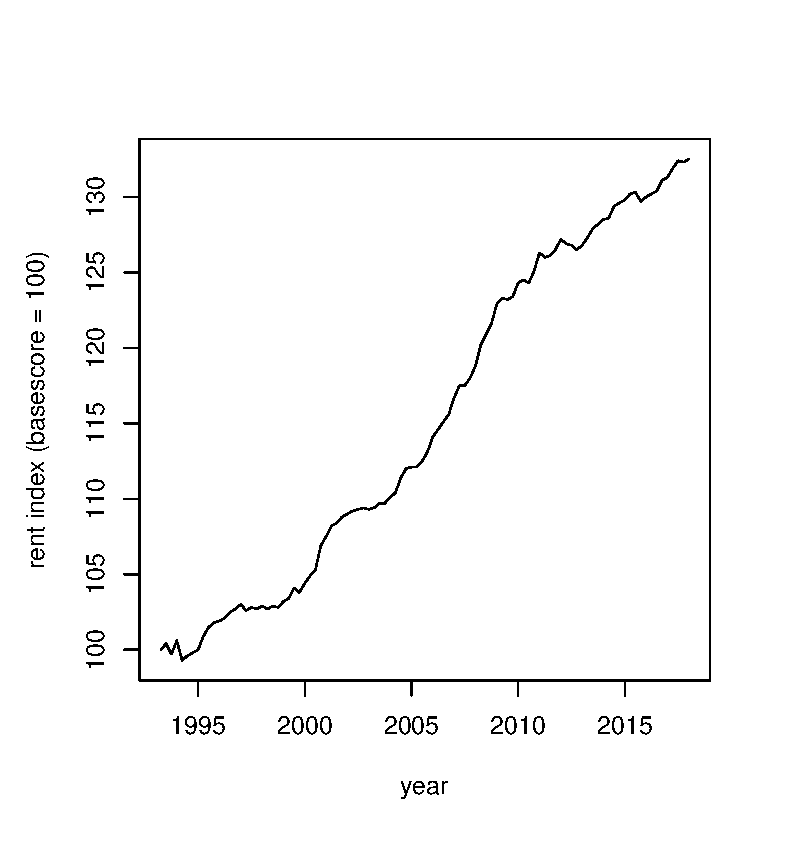
\includegraphics[angle=0,
width=0.7\textwidth]{indiceloyers_timeseries}
\caption{Swiss rent index, years 1993 to 2018\label{fig:indiceloyers_timeseries}}
\end{figure}

As we can see in figure~\ref{fig:indiceloyers_timeseries} a trend is obviously visible, however we cannot be that sure if it doesn't exist a seasonal component either. Therefore in the next step we check first whether they are possible seasonal components, afterwards we will fit several models to get rid of the trend. 

\begin{figure}[!htb]
\centering
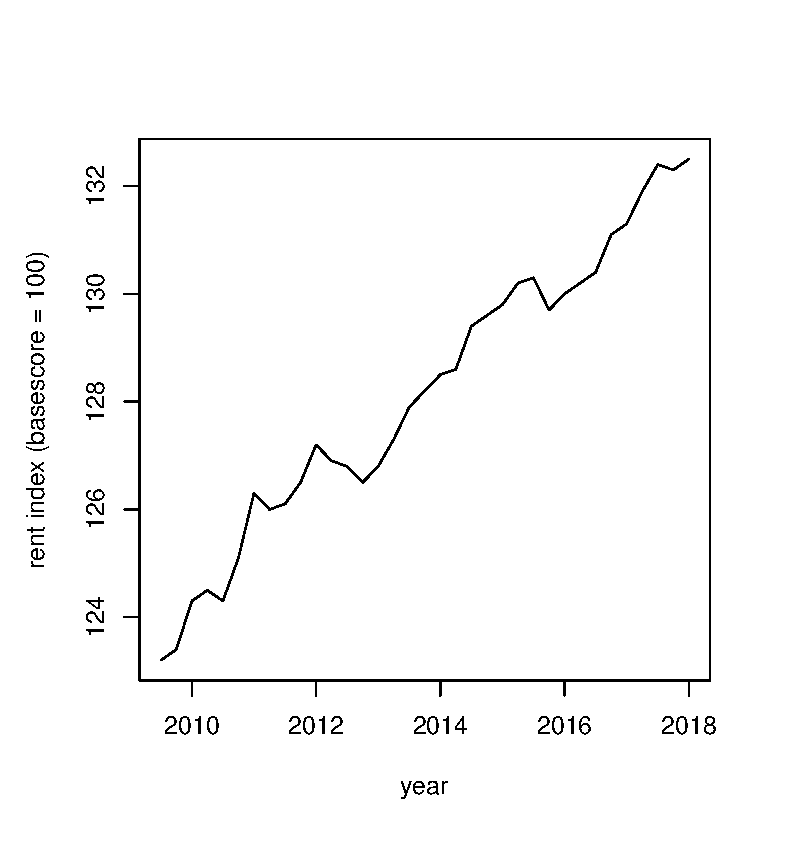
\includegraphics[angle=0,
width=0.7\textwidth]{indiceloyers_test}
\caption{Swiss rent index, years 2009 to 2018\label{fig:indiceloyers_test}}
\end{figure}
\begin{figure}[!htb]
\centering
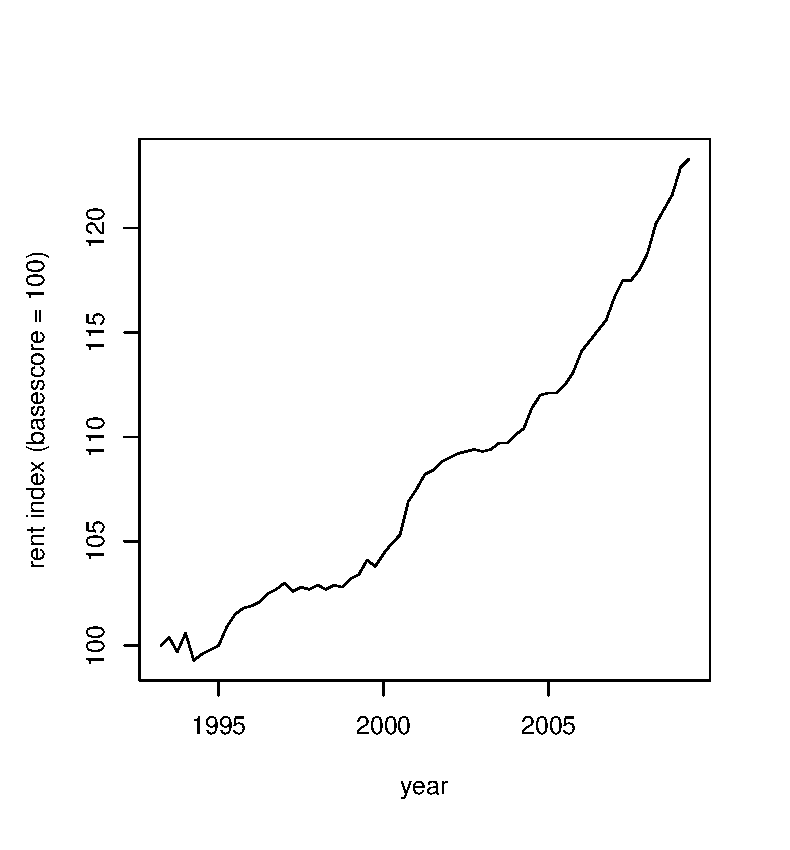
\includegraphics[angle=0,
width=0.7\textwidth]{indiceloyers_train}
\caption{Swiss Rent index, years 1993 to 2009\label{fig:indiceloyers_train}}
\end{figure}


\subsection{Check for Seasonality}
Since the data are collected quarterly we use a linear regression model with d=4 dummy predictors to check for significant seasonal coefficients, meaning a dummy for every quarter (LN1-2, p. 36). 
\begin{figure}[!htb]
\centering
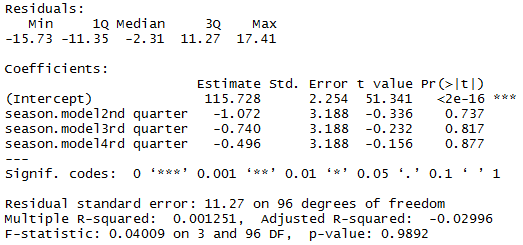
\includegraphics[angle=0,
width=0.7\textwidth]{summary_seasonmodel}
\caption{summary statistics of the fitted seasonal model\label{fig:summary_seasonmodel}}
\end{figure}
As we can see from figure~\ref{fig:summary_seasonmodel} none of the estimated seasonal coefficients are significant. We can be sure now that they are no seasonal impacts on our data, hence what remains is to eliminate the trend. In the absence of a seasonal component our model becomes the following \cite[p.~24]{bd02}:
\begin{equation}
X_t = m_t + Y_t, \text{t = 1,...,n,} 
\\where EY_t = 0
\end{equation} 

\subsection{Trend Elimination by fitting polynomial models}
As we have shown in the above subsection, we don't have to get rid of seasonal components, nevertheless we have to get rid of the obvious trend. Whilst the time series \ref{fig:indiceloyers_timeseries} indicates a probable polynomial trend, especially a linear one, we are starting by fitting different polynomial trends by ordinary least squares estimation. We are going to fit a linear trend, a quadratic trend, a cubic trend as well as a logarithmic trend. The latter  helps to transform a potentially exponential increase in the rent index into a linear trend, even though at first sight the time series \ref{fig:indiceloyers_timeseries} looks more like a linear than an exponential trend, we are going to test for a logarithmic trend either.
\\
\begin{figure}[!htb]
\centering
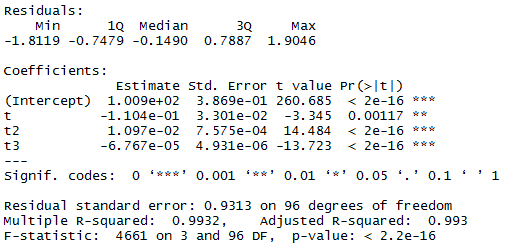
\includegraphics[angle=0,
width=0.7\textwidth]{summary_cubicmodel}
\caption{summary statistics of the fitted cubic model\label{fig:summary_cubicmodel}}
\end{figure}
The coefficients in all 4 models are highly significant and with an $R^2$-Value of 98 to 99 percent (meaning that the models would be able to explain up to 98percent (99percent respectively) of the variance), the linear, the quadratic and the cubic model would explain our data extremely well. This can can be well seen at the cubic model's example in \ref{fig:summary_cubicmodel}. The logarithmic model shows a bit less explanatory power with an $R^2$-Value of 0.72, even though its coefficient is highly significant as well. However we have to be careful with the interpretation of the p-values since this regression models assume independence of the observations whereas our purpose of the summary statistics of fitted linear models is a different one: to use residuals in order to construct a stationary time series (Brooks Davis p. xy). 

\subsubsection{Diagnostics of the fitted polynomial trends}

\begin{figure}[!htb]
\centering
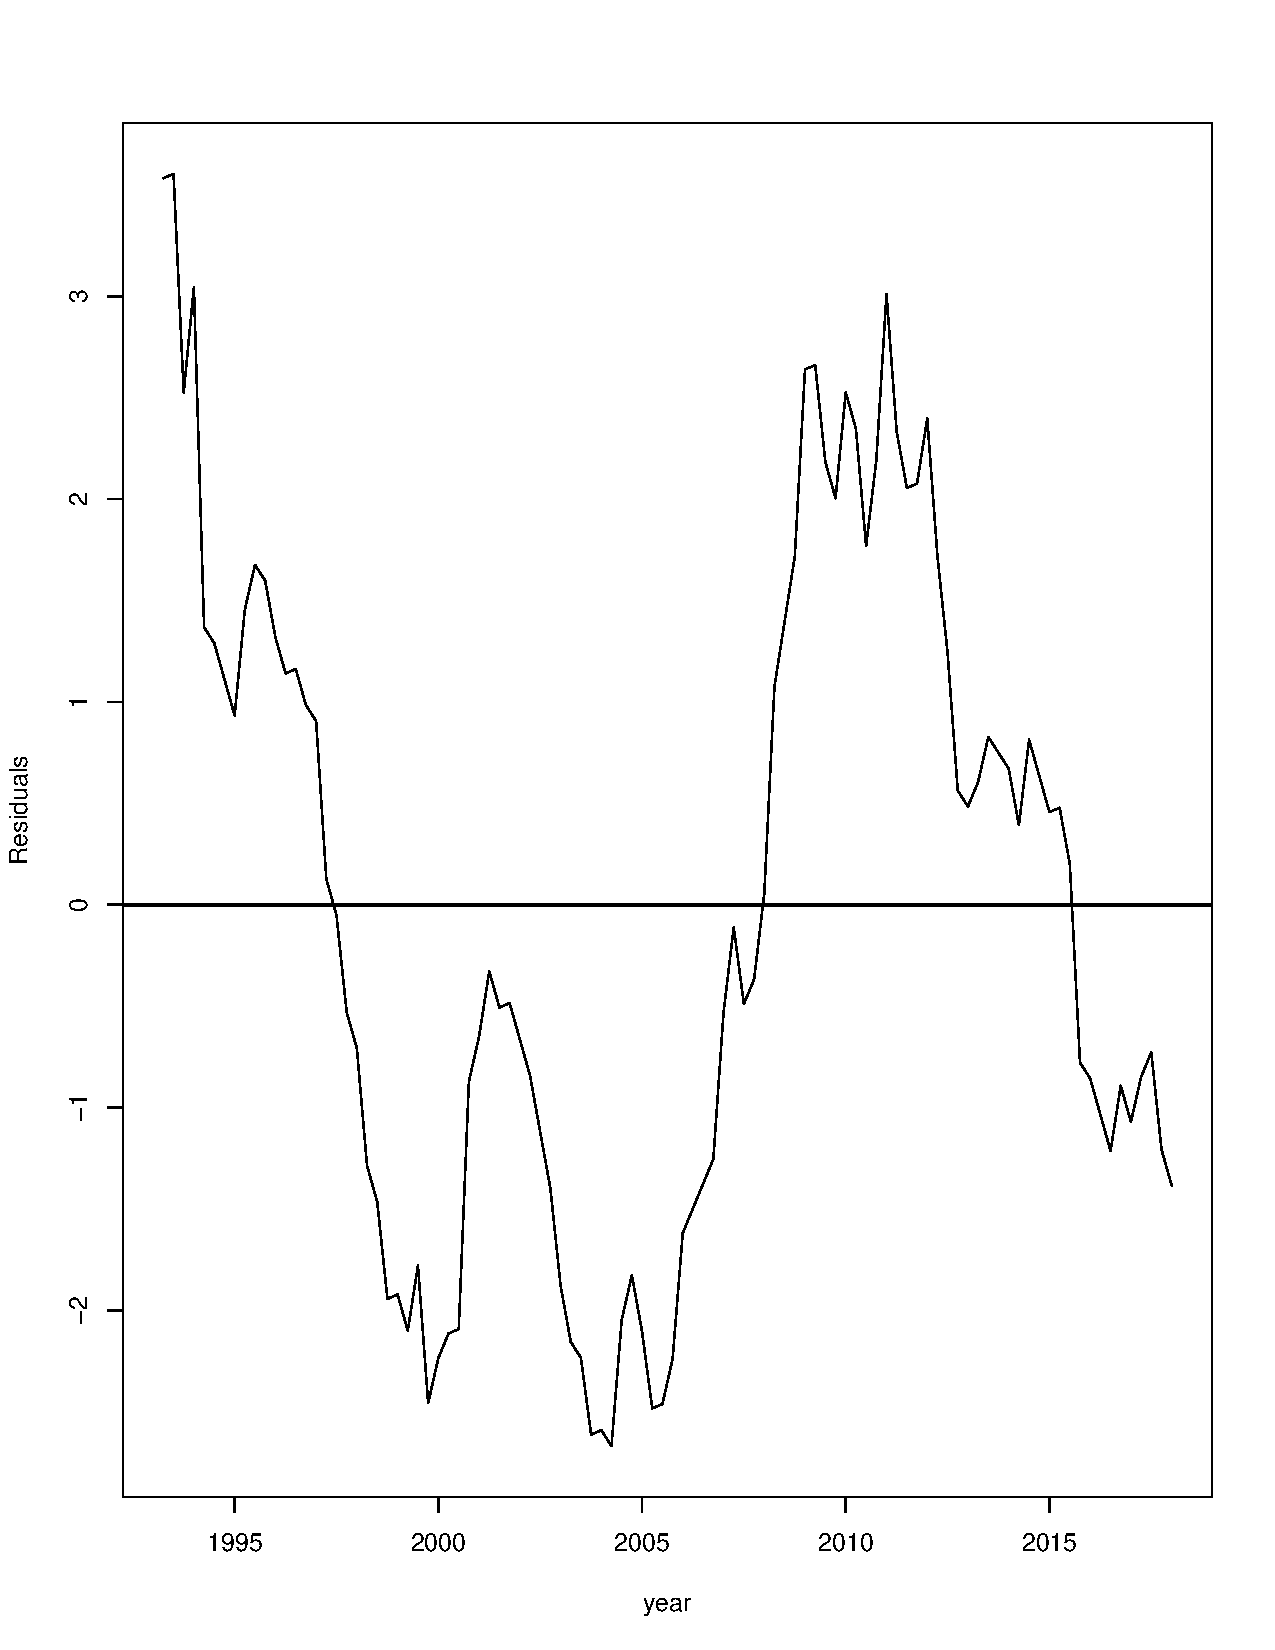
\includegraphics[angle=0,
width=0.5\textwidth]{resid_linearmodel}
\caption{Residuals of a fitted linear model
\label{fig:resid_linearmodel}}
\end{figure}

\begin{figure}[!htb]
\centering
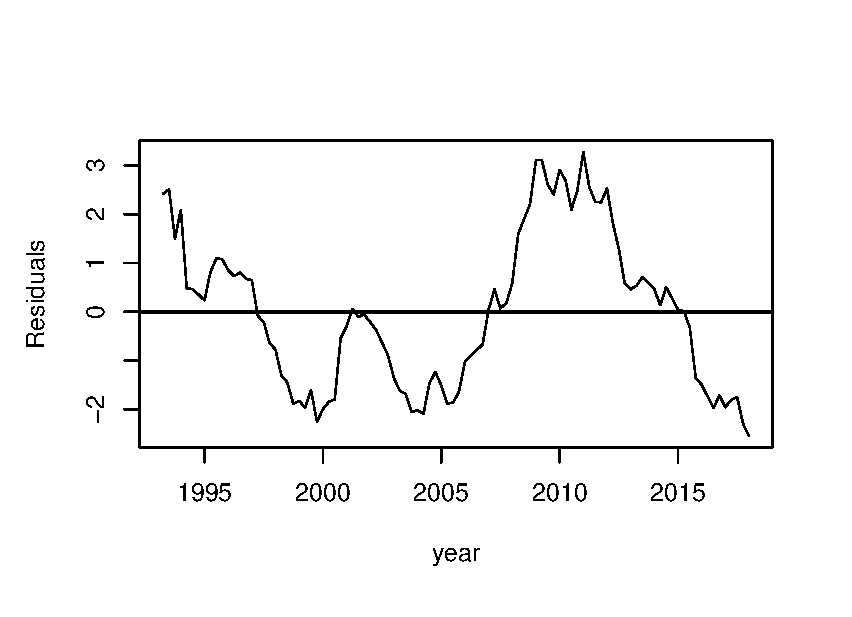
\includegraphics[angle=0,
width=0.5\textwidth]{resid_quadraticmodel}
\caption{Residuals of a fitted quadratic model
\label{fig:resid_quadraticmodel}}
\end{figure}

\begin{figure}[!htb]
\centering
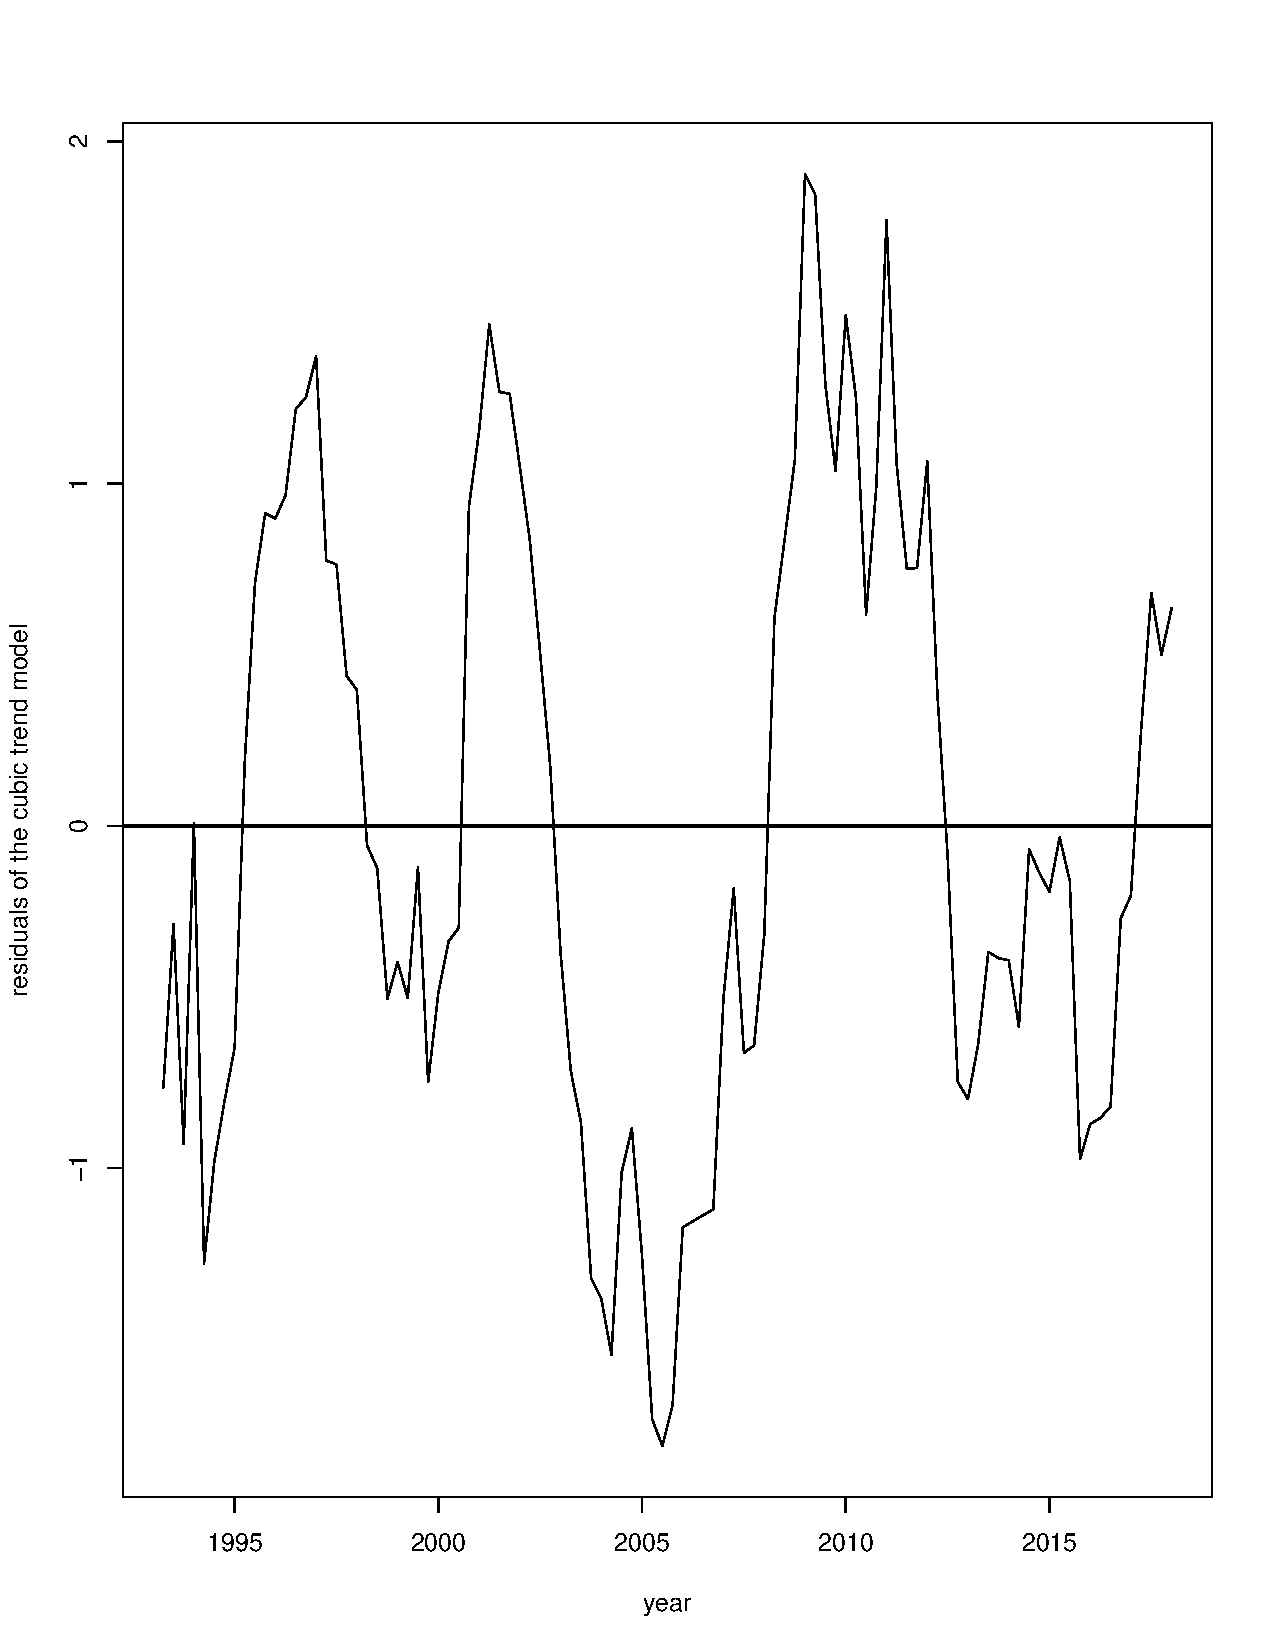
\includegraphics[angle=0,
width=0.5\textwidth]{resid_cubicmodel}
\caption{Residuals of a fitted cubic model
\label{fig:resid_cubicmodel}}
\end{figure}

\begin{figure}[!htb]
\centering
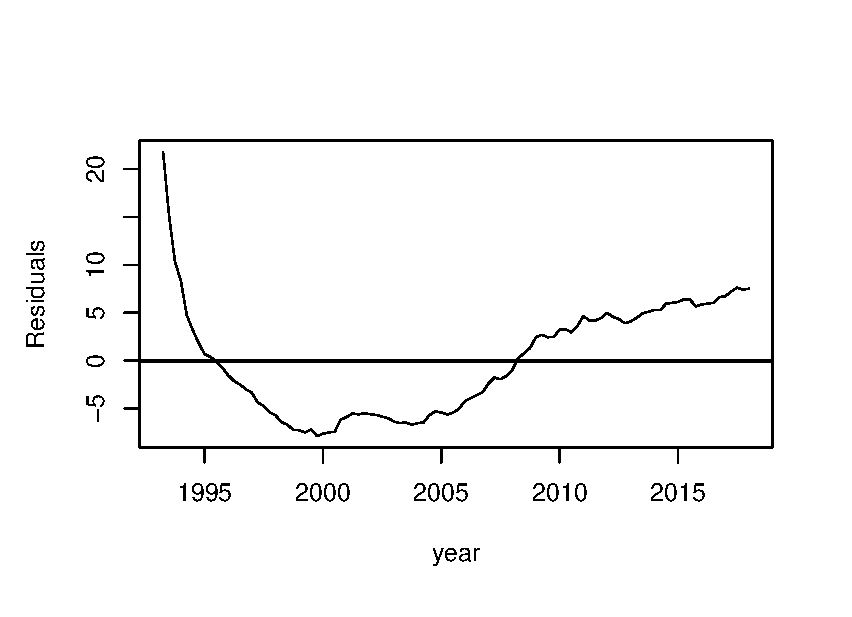
\includegraphics[angle=0,
width=0.5\textwidth]{resid_logmodel}
\caption{Residuals of a fitted logarithmic model
\label{fig:resid_logmodel}}
\end{figure}
Unfortunately the plots for polynomial trend elimination don't show any stationarity, as the series wanders up and down for quite some periods. as we can derive from the four figure~\ref{fig:resid_linearmodel}, figure~\ref{fig:resid_quadraticmodel}, figure~\ref{fig:resid_cubicmodel} and figure~\ref{fig:resid_logmodel}. The four plots show large covariances and their residuals are evidently depending on time $t$, meaning non-stationary.
\\
\begin{figure}[!htb]
\centering
\includegraphics[angle=0,
width=0.5\textwidth]{acf_cubicmodel}
\caption{Sample autocorrelation function of the cubic model
\label{fig:acf_cubicmodel}}
\end{figure}
Furthermore from the ACF-plot (figure~\ref{fig:acf_cubicmodel}) and the PACF-plot (figure~\ref{fig:pacf_cubicmodel}) exemplified on the cubic model, we can see that there are a lot of significant lags outside the 95-percent-confidence bounds of $+/-1.96sqrt{n}$.  These bars don't die out quickly. So the $Rho_hat$ can be a useful indicator of non-stationarity \cite[p.~21]{bd02}. Hence, we can conclude our covariances depend on time and therefore the series is non-stationary. similar time-depending patterns hold true for the autocovariance-functions of our other polynomial trend models: the linear, the quadratic and the logarithmic model. 
\\In addition we get numerical evidence from three different tests checking for stationarity or independence of the observations, respectively. First the Ljung-Box test examines whether there is significant evidence for non-zero correlations at lags 1-40. Small p-values (i.e., less than 0.05) suggest that the residuals are independent. The Ljung-Box Hypothesis0 of independence has to be rejected for all four polynomial models so far (TODO show the 4 p-values). The Augmented Dickie-Fuller test and the Kwiatkowski-Phillips-Schmidt-Shin (KPSS) test provide as well strong evidence for non-stationary for all 4 polynomial models (TODO show the 4 p-values). Even though we have to keep in mind the low power of Dickie-Fuller Test for our purposes given the fact this test assumes a AR-Process, about which we cannot be too sure  yet. 
\\ The following figure~\ref{fig:overview_polynomial} shows an overview over the tests considering non-stationarity and independence of the observations.

Since the fitted polynomial models doesn't help us to give a stationary series we will consequently try to differentiate our data in the next subsection.

\subsection{Trend Elimination by differencing}

Since it is not possible to obtain a stationary time series by fitting polynomial trends we have to use different methods. Hence, we try to eliminate the trend by differencing the data at different lags (1, 2, 3 and 4) in order to generate a noise sequence and therefore get a stationary series \cite[p.~35]{bd02}). 


The following figure~\ref{fig:diff1_timeseries}, figure~\ref{fig:diff2_timeseries}, figure~\ref{fig:diff3_timeseries} and figure~\ref{fig:diff4_timeseries} show the differenced series derived from the quarterly rents for each lag = 1, 2, 3 and 4.
\begin{figure}[!htb]
\centering
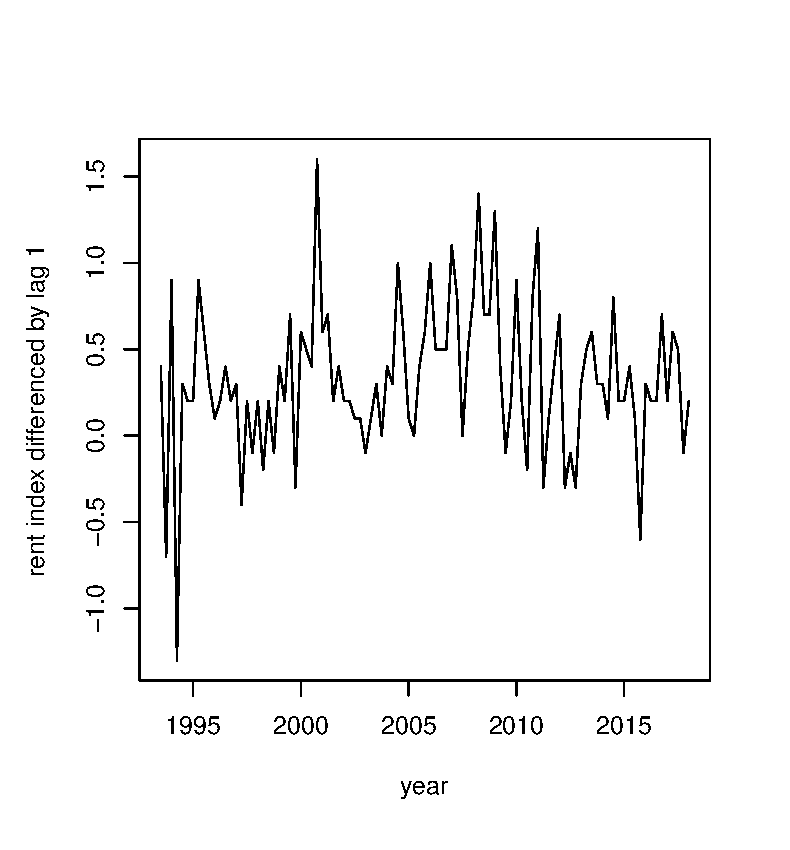
\includegraphics[angle=0,
width=0.5\textwidth]{diff1_timeseries}
\caption{once-differenced rent index
\label{fig:diff1_timeseries}}
\end{figure}
\begin{figure}[!htb]
\centering
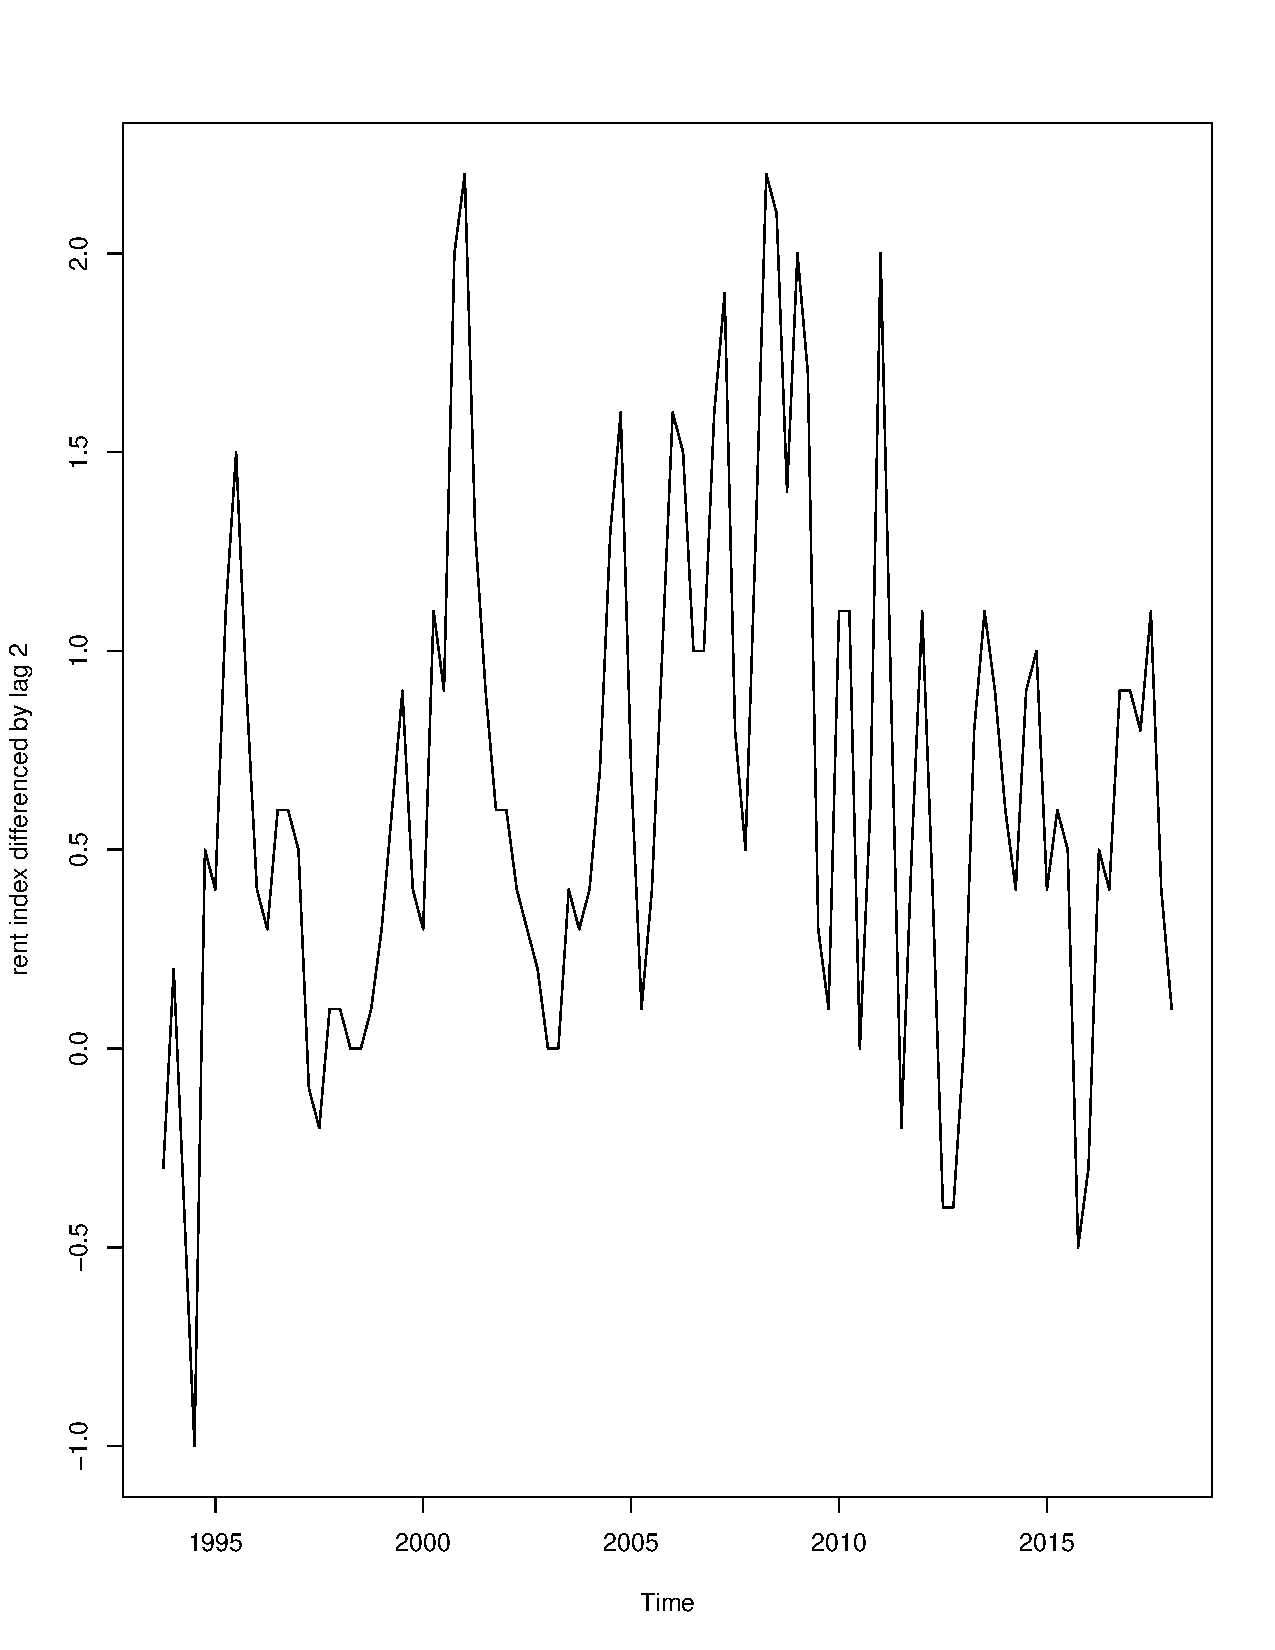
\includegraphics[angle=0,
width=0.5\textwidth]{diff2_timeseries}
\caption{twice-differenced rent index
\label{fig:diff2_timeseries}}
\end{figure}
\begin{figure}[!htb]
\centering
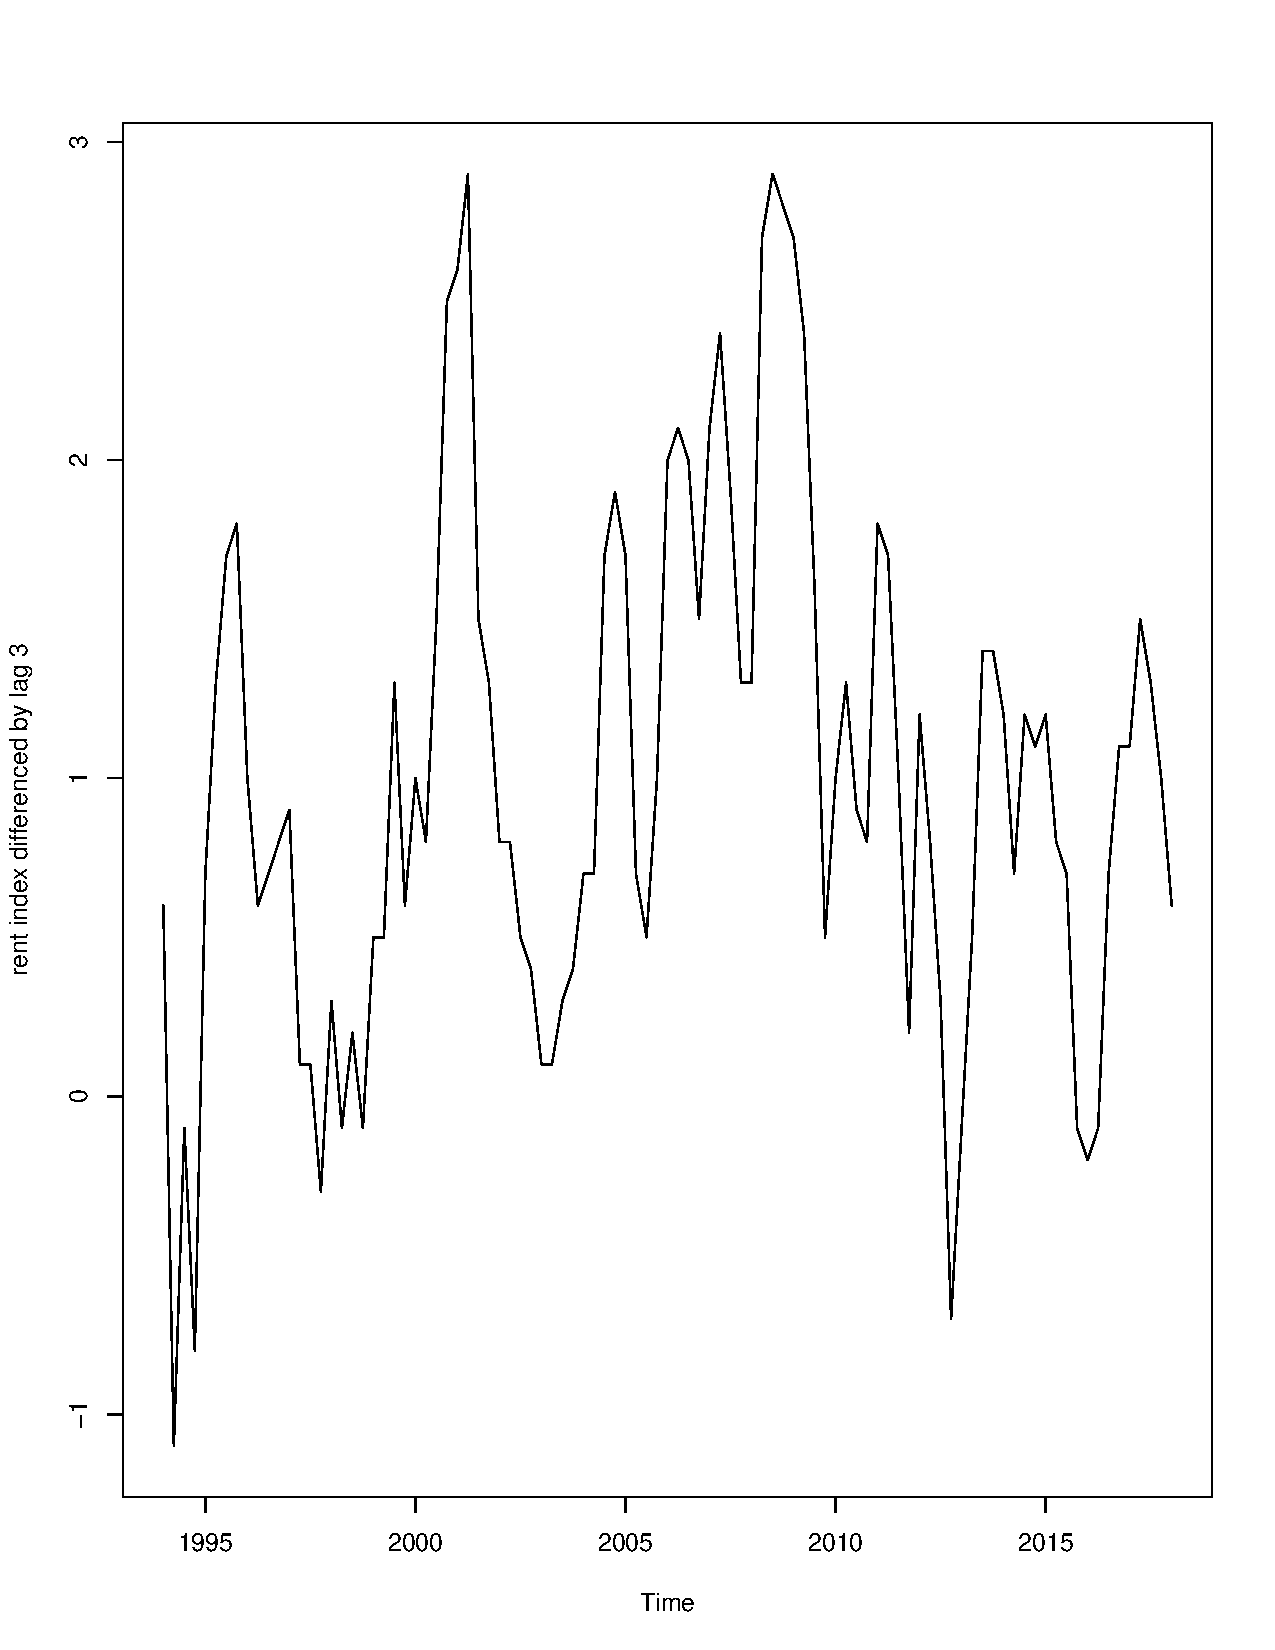
\includegraphics[angle=0,
width=0.5\textwidth]{diff3_timeseries}
\caption{triple-differenced rent index
\label{fig:diff3_timeseries}}
\end{figure}
\begin{figure}[!htb]
\centering
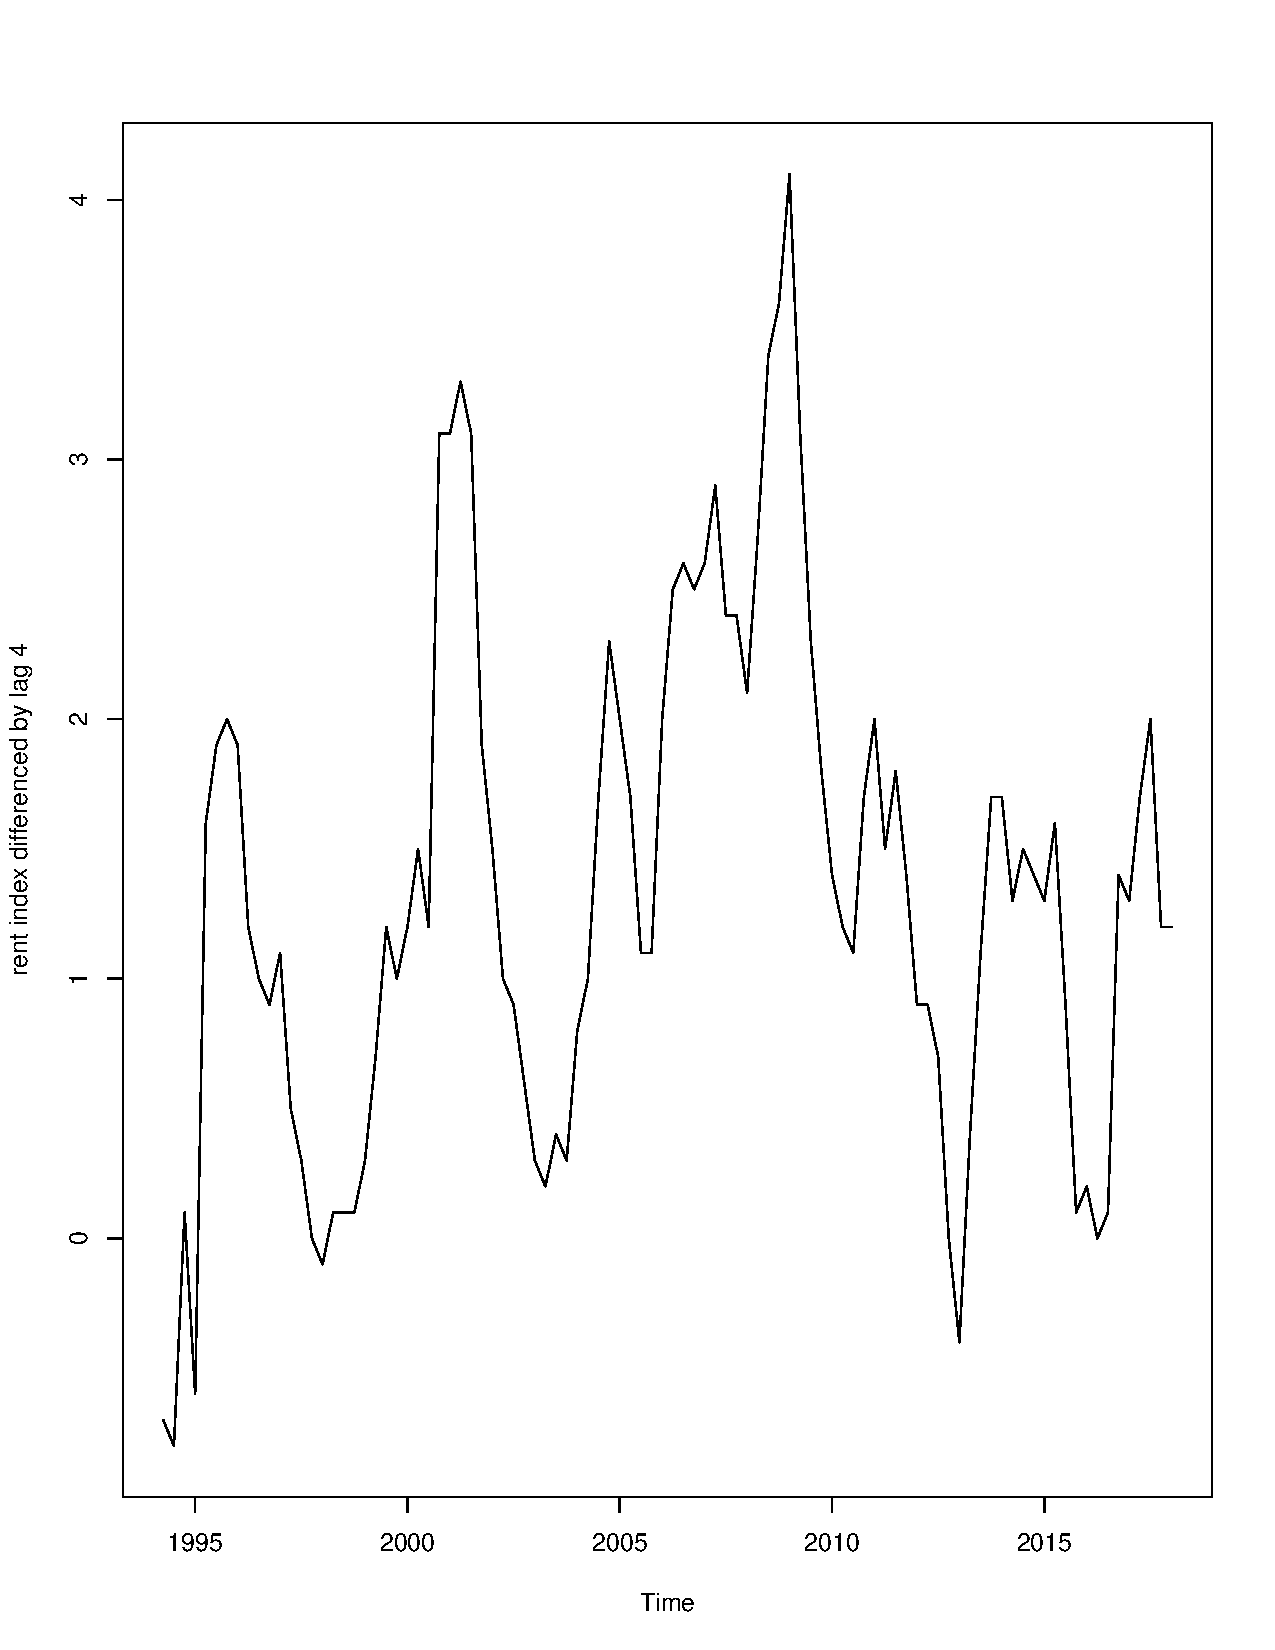
\includegraphics[angle=0,
width=0.5\textwidth]{diff4_timeseries}
\caption{quadruple-differenced rent index
\label{fig:diff4_timeseries}}
\end{figure}
For the first two models we were succesfully able to generate stationary residuals which don't depend on time. However figure~\ref{fig:diff1_timeseries} shows mostly patterns of a white noise which is not what we intended since in case of a white-noise-process prediction quality is poor (Expectation of $x_n+1$ would be 0 in case of a mean-centered series). This white-noise patterns is as well indicated by the sample autocorrelation function of the once-differenced series where all lags up to 40 fall well within the bounds of $+/-1.96sqrt{100}$ (brooks davis p.39)  (see figure~\ref{fig:diff1_acf}) . To conclude, the once-differenced series is to versatile and contains too much randomness to get good predictions.
\begin{figure}[!htb]
\centering
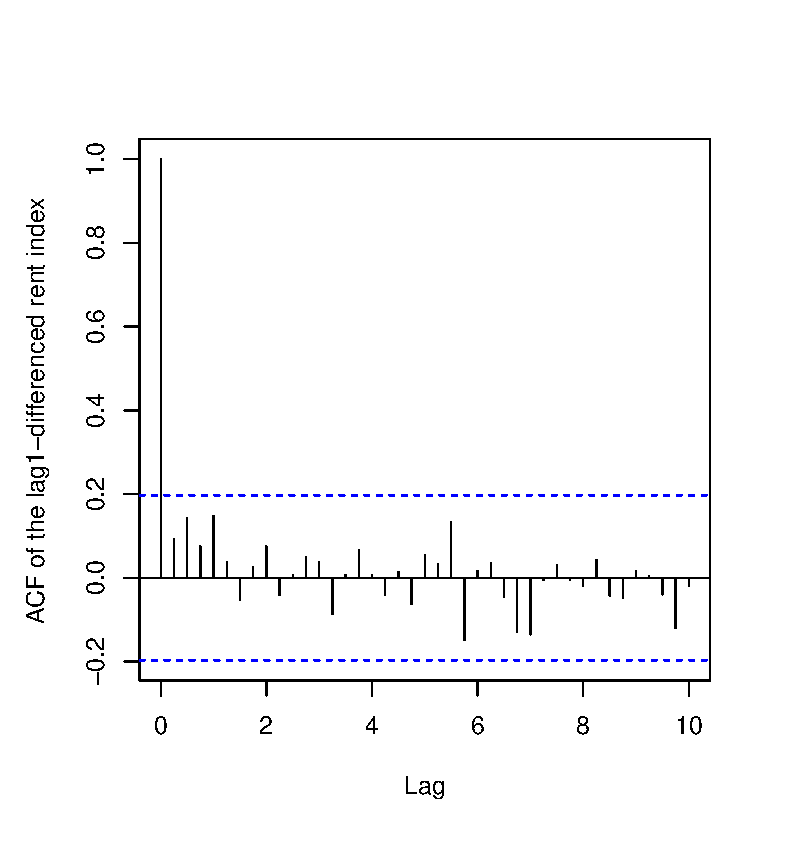
\includegraphics[angle=0,
width=0.5\textwidth]{diff1_acf}
\caption{auto-correlation function of the once-differenced series
\label{fig:diff1_acf}}
\end{figure}
The Ljung-Box-Test \citep{LjungBox78} indicates a p-value of 0.35, meaning that we cannot reject the iid-Hypothesis $H_0$ that there is independence between the observations. Therefore The Ljung-Box-Test emphasizes furthermore the independence of the values and the white-noise-patterns of the once-differenced series. Since white-noise would mean E0 and Variance sigma no more modelling would be necessary which is not what we want as we evoked in the introduction to this section

\subsubsection{Diagnostics of the twice-differenced series}
\begin{figure}[!htb]
\centering
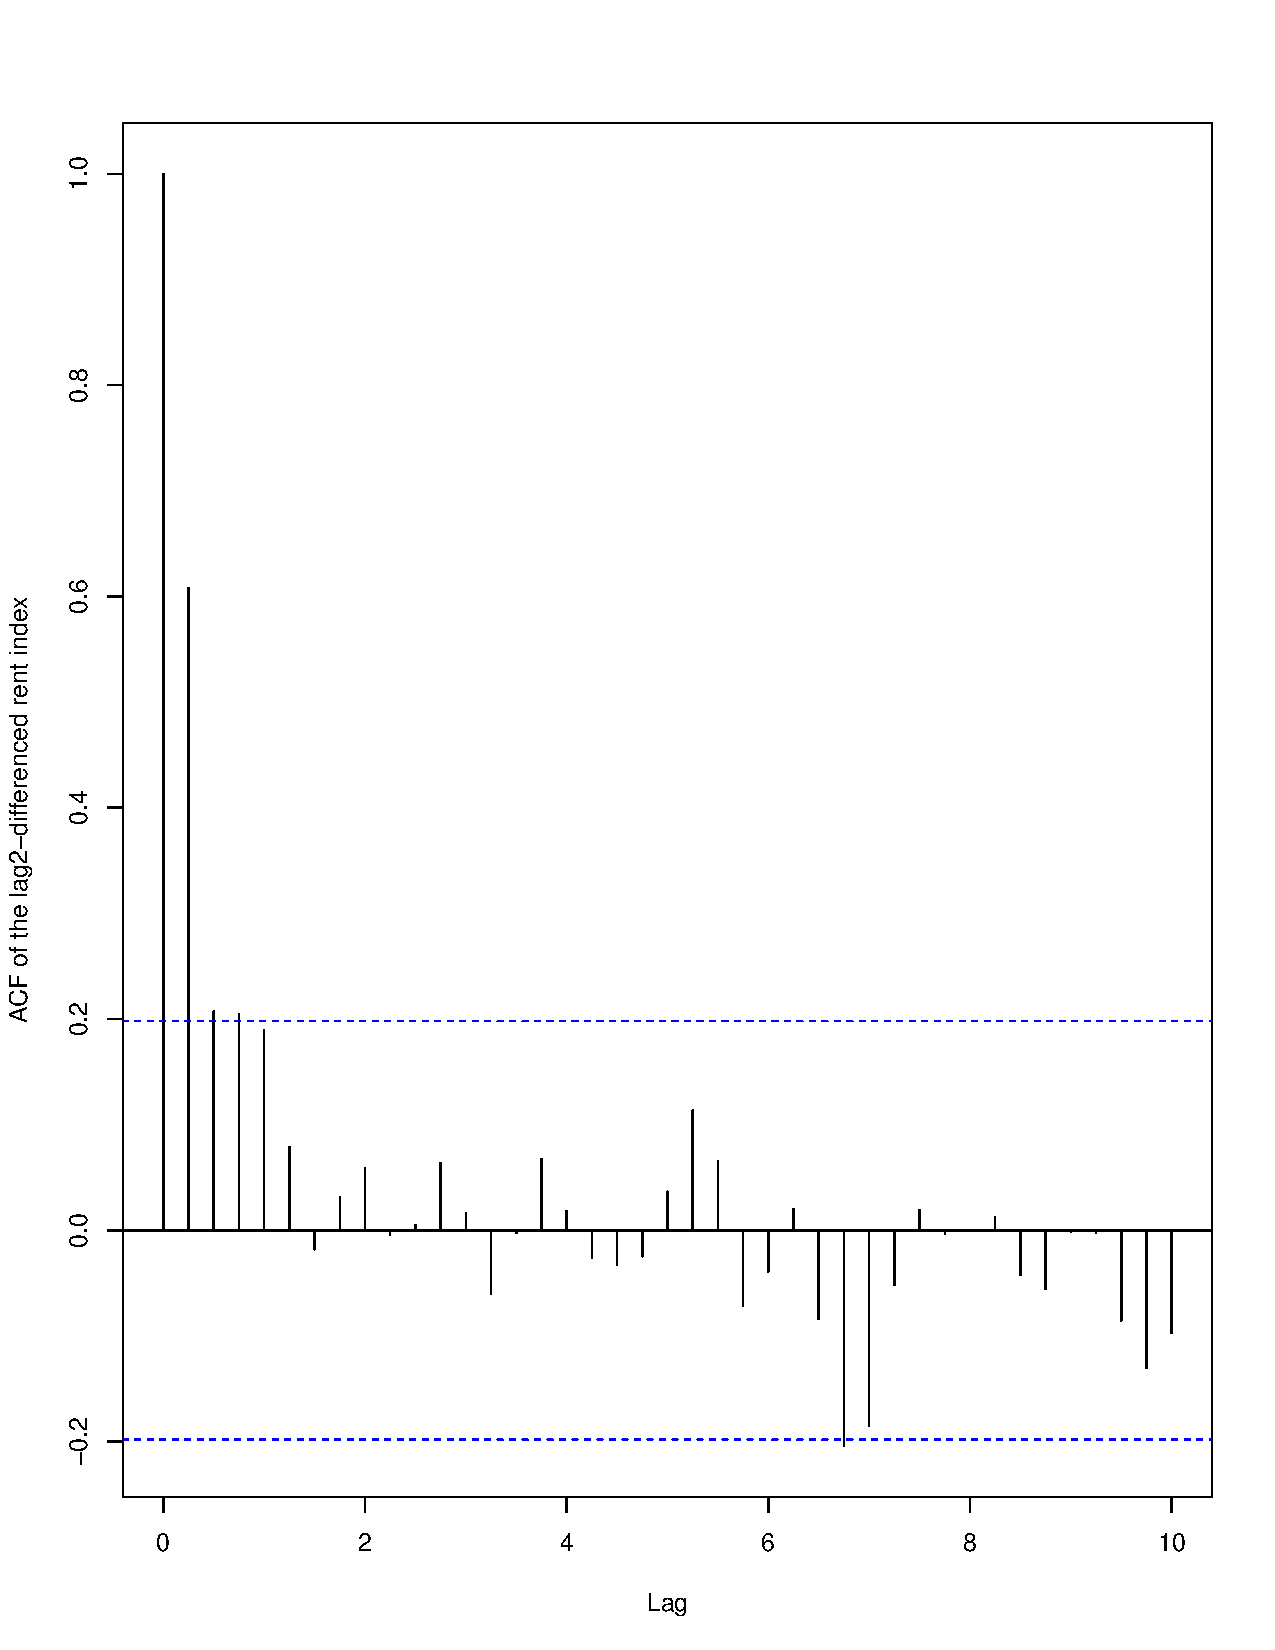
\includegraphics[angle=0,
width=0.5\textwidth]{diff2_acf}
\caption{auto-correlation function of the twice-differenced series
\label{fig:diff2_acf}}
\end{figure}
\begin{figure}[!htb]
\centering
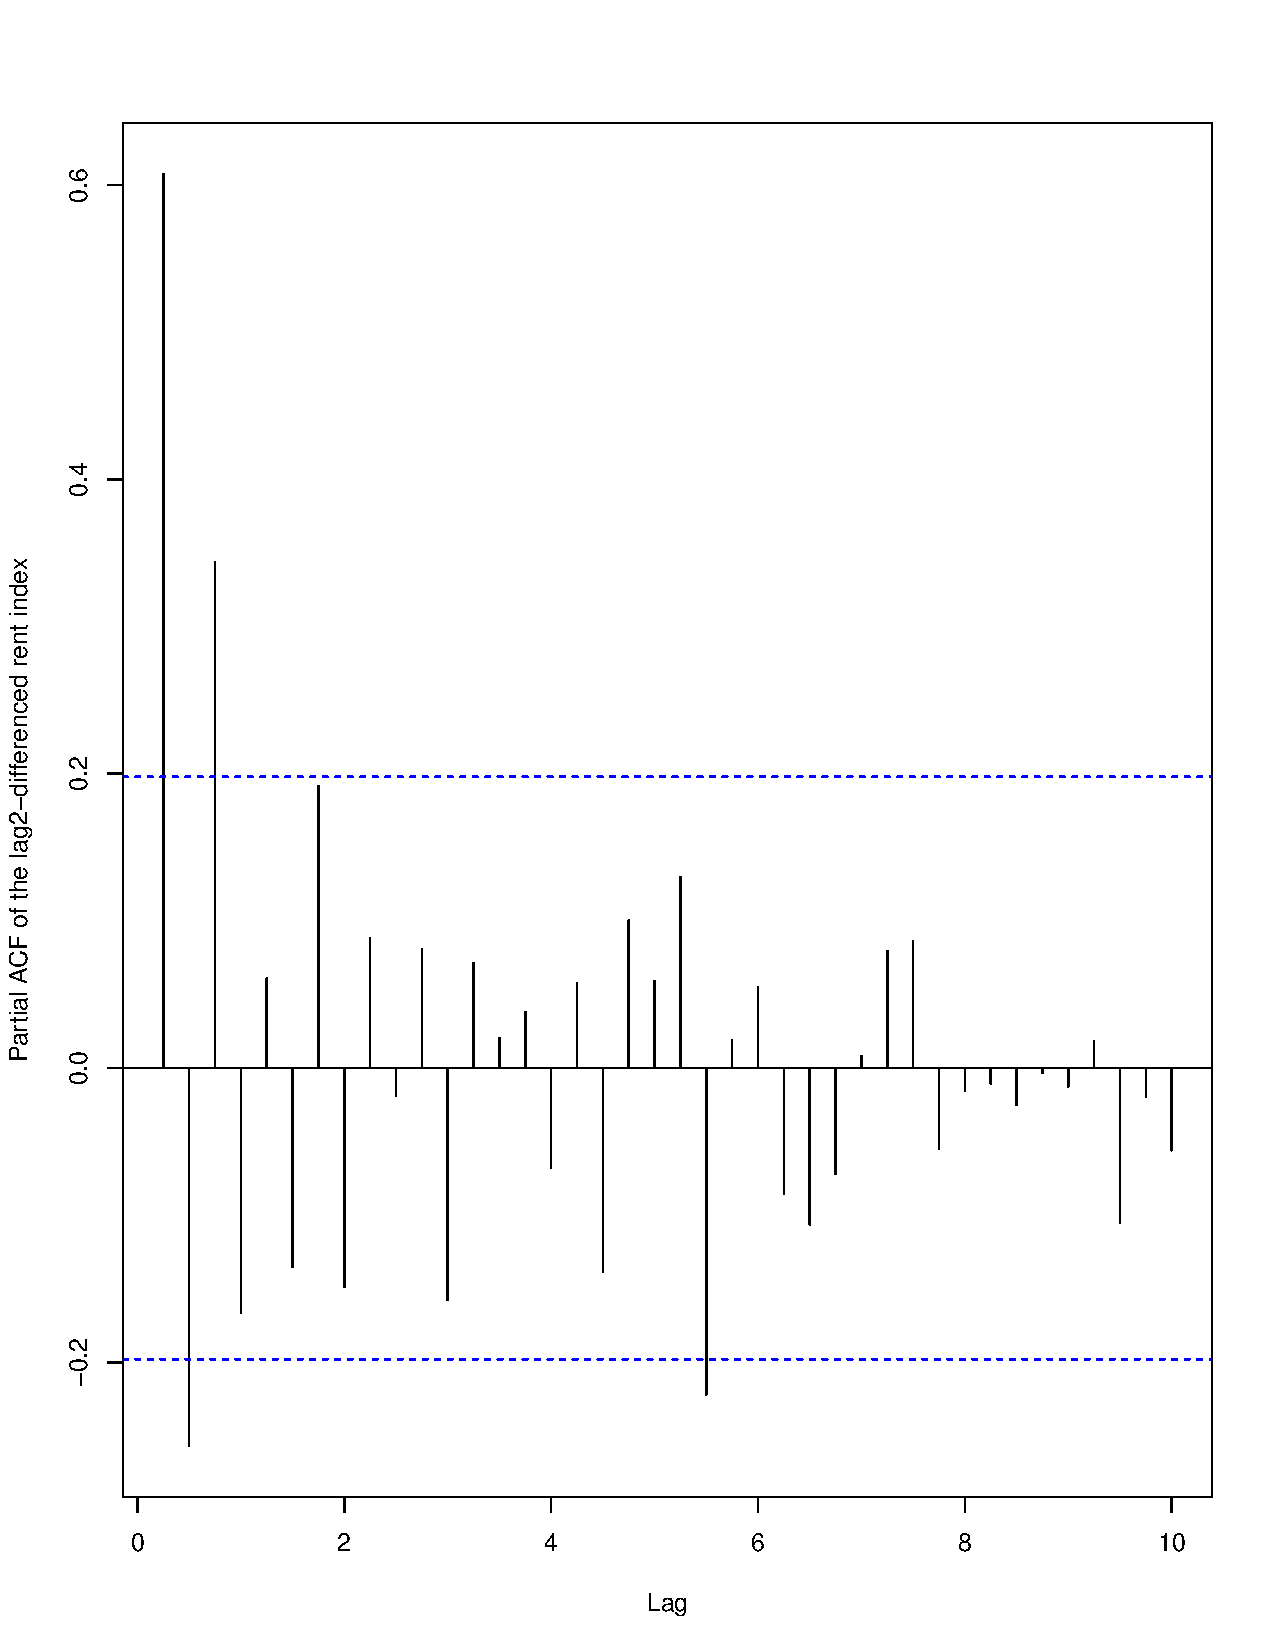
\includegraphics[angle=0,
width=0.5\textwidth]{diff2_pacf}
\caption{Partial auto-correlation function of the twice-differenced series
\label{fig:diff2_pacf}}
\end{figure}
In order to get better predictions and forecasting power than with pure white-noise-residuals seen in the once-differenced series, we now go for a twice-differenced model. Indeed our twice-differenced model doesn't show anymore iid-noisy patterns, indicating by the sample ACF (see figure~\ref{fig:diff2_acf} which shows at least a correlation at lag1 and some other lags are touching the $+/-1.96sqrt{n=100}$ - 95percent-confidence-bounds. The ACF of the twice-differenced model shows only a few significant lags which die out quickly. This is a good sign, meaning that on one hand we have correlations which are needed to do prediction, on the other hand the covariance is not too large to be considered time-dependant and therefore we can conclude to have a stationary series.
Cross-validation with a test data set considering only the last 35 of the 100 observations (see figure~\ref{fig:diff2_testset} above) confirms furthermore the non-stationary character of the twice-differenced-model 
Box.test(d2.indiceloyers.test, lag=2, type="Ljung-Box") p-value of 0.033 suggests the data are (time-)independent
adf.test(d2.indiceloyers.test, alternative = "stationary", k=2)  H0 of non-stationarity cannot be rejected which is not a problem, that could be due to lack of observations
kpss.test(d2.indiceloyers.test)  with a p-value>0.05 the test data seems to be stationary aswell
the data of the first segment's (1993 to 2009) twice-differenced series show independent observations as well (see figure~\ref{fig:diff2_trainingset}), however we can see a slightly slower increase in the segment from 2009 to 2018 indicating that in the years from 1993 to 2009 the growth in rental prices was higher than in the years in the second's segment which begins from 2009. that can be explained by the big baisse in the early 90ies, starting from a lower initial point and better conjunctural perspectives the increase was stronger, whilst from 2009 on the growth in rental prices slowed down, which can be very well explained by the US subprime crises beginning in the year 2008 followed by a long-taking global recession.
\begin{figure}[!htb]
\centering
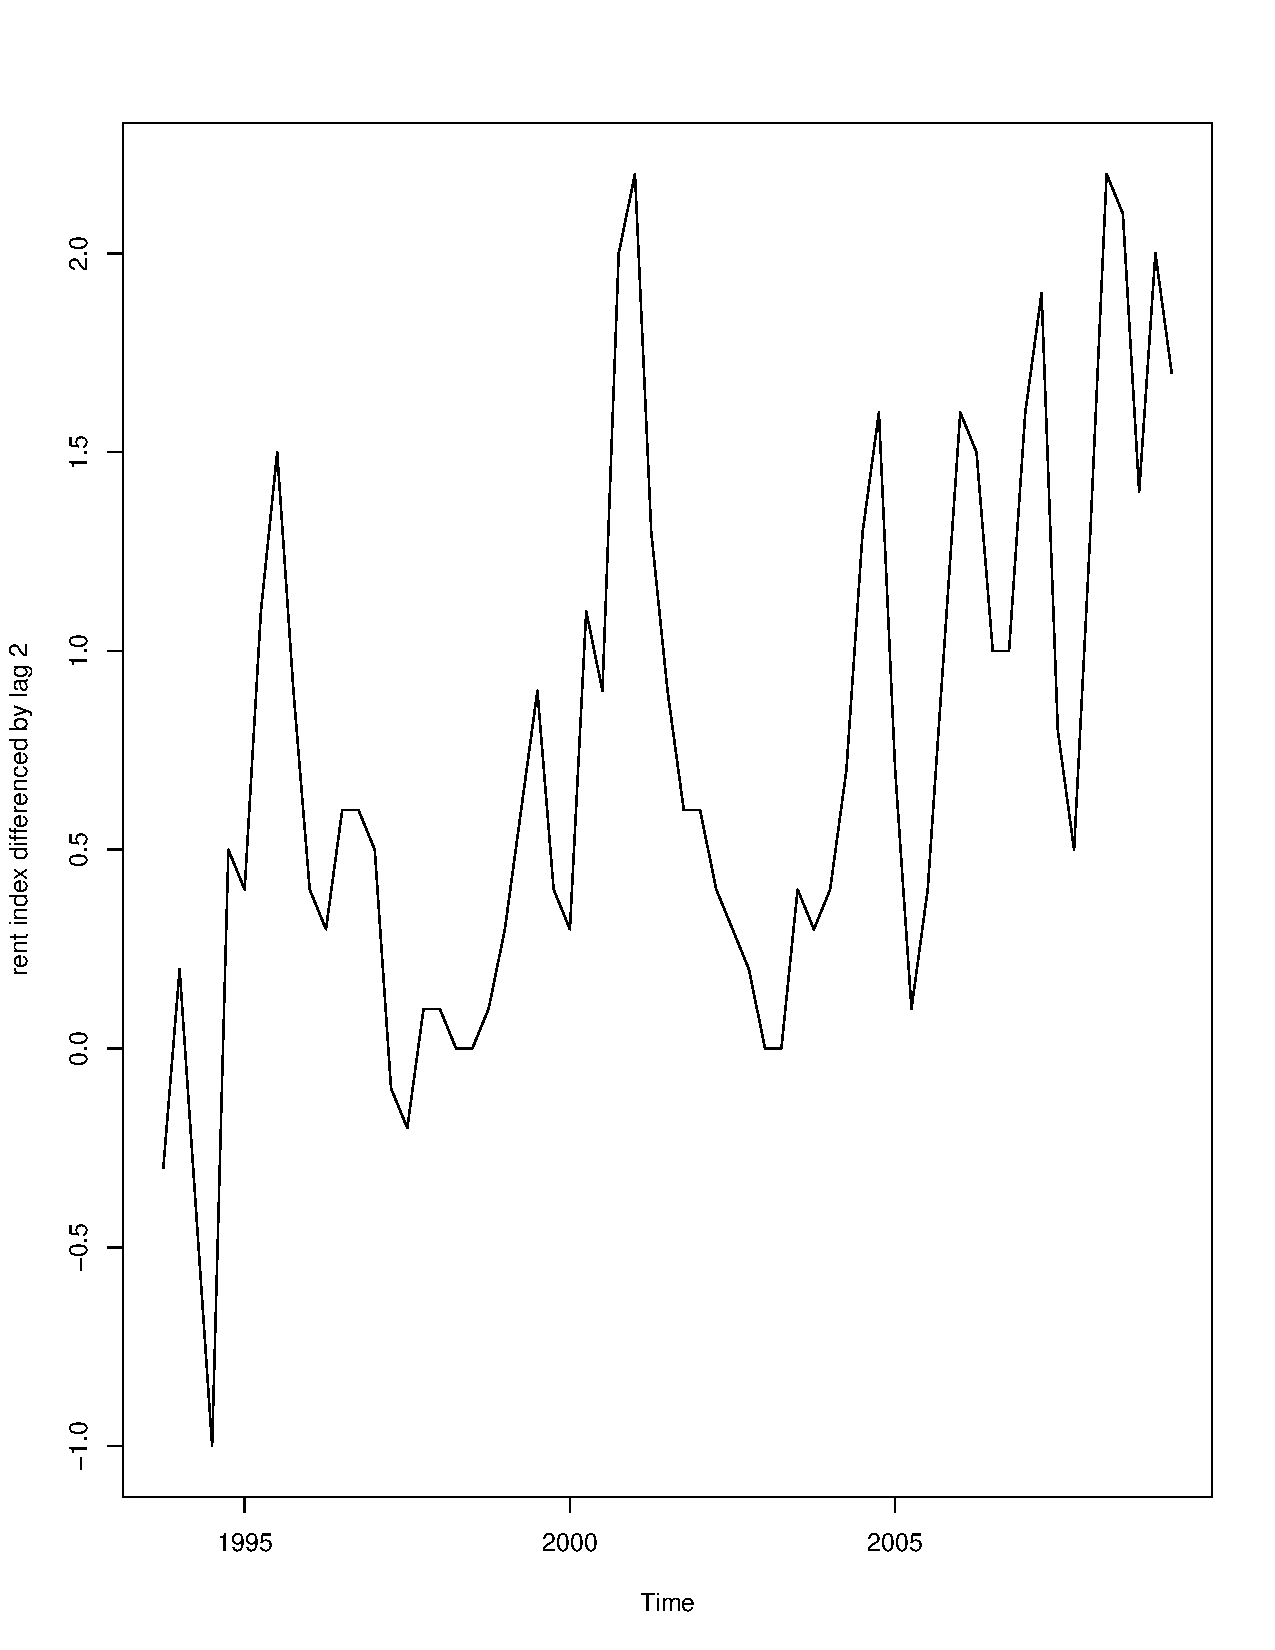
\includegraphics[angle=0,
width=0.5\textwidth]{diff2_trainingset}
\caption{twice-differenced series from 1993 to 2009
\label{fig:diff2_trainingset}}
\end{figure}
\begin{figure}[!htb]
\centering
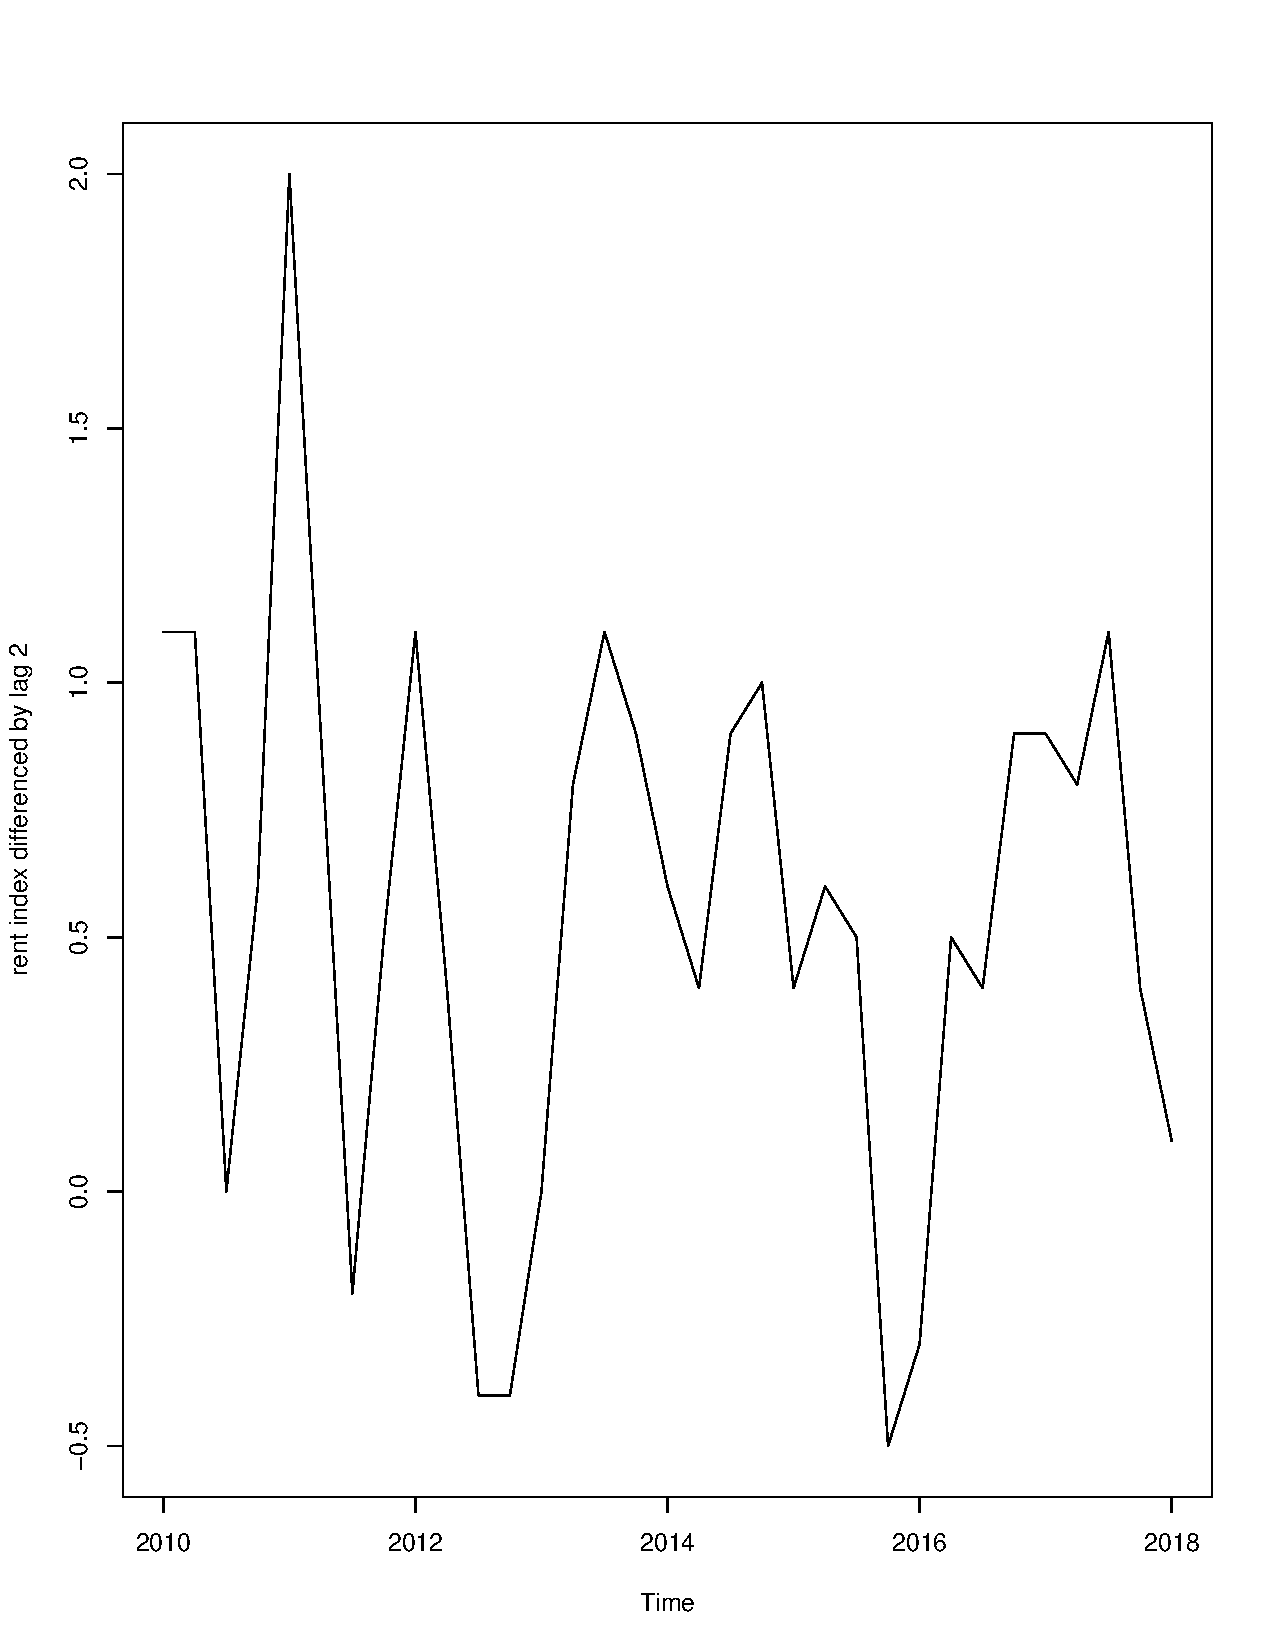
\includegraphics[angle=0,
width=0.5\textwidth]{diff2_testset}
\caption{twice-differenced series from 2009 to 2018
\label{fig:diff2_testset}}
\end{figure} 

\subsubsection{Diagnostics of the triple-/quadruple-differenced series}
Differencing by lag 3 and 4 is not appropriate neither since there is too much autocorrelation showed by the ACF a lot of bars outside the $+/-1.96sqrt{100}$ - bounds.

To conclude, our transformation should be the twice-differenced series, since the once-differenced series is too white-noisy and the triple/quadruple-differenced series show too large covariances (time-dependence/nonstationarity). Finally to continue fitting and testing a model we center our twice-differenced series by subtracting the mean in order to...

\section{Fitting and Testing the Model} \label{Fitting and Testing the Model}
\subsection{preliminary estimation and order selection}
From the sample ACF and PACF (figure~\ref{fig:diff2_acf}) (figure~\ref{fig:diff2_pacf}) of our centered twice-differenced model we can see in the ACF-plot a highly significant spike at lag 1 and the following bars dying out quickly, lying inside the 95percent-confidence – bounds (with bars at lag 2 and 3 slightly touching the 95percent-confidence-bounds). The combined view of the PACF-plot with its exponentially decreasing patterns (in absolute values) and the 1 spike in the ACF-plot let us suggest an MA(1)-model could fit our data quite well.
However, since we are operating with only 100 observations, one can not exclude that there could be underlying exponentially decreasing patterns in the ACF plot as well. Exponential decrease (in absolute values) in both ACF and PACF plot would rather suggest an ARMA-model then. Since we’re following an conservative approach we are going to test for MA(1) as well as for ARMA-model. In opposition to exclusive AR(q)- or exclusive MA(p)-models where we can derive the order of p or q from the number of spikes in the ACF and PACF plot, the same holds not true to guess the orders of p and q for ARMA-models. Therefore in case of ARMA-models we have to choose the order of p and q in another way, by comparing models with different p and q and decide which performs best in terms of the corrected Akaike Information Criterion (AICC).
The following matrix (figure~\ref{fig:aicc_matrix}) shows the AICC for different orders of p and q. The one with the lowest value performs best \citep{aic86}. We can see that an MA(1)-model gives us the lowest AICC-value which is very well confirmed by the ACF/PACF plots. However, since the sample ACF and PACF, as mentioned above, could possibly both decrease exponentially (in absolute values), we are going fit as well an ARMA(1,1) and ARMA(1,2) model, since both of them show very low AICC-values, too (see AICC-Matrix in figure).
Estimation of the model candidates
We estimate our three model candidates by the arima function . This function implies a rough estimation by (hannan rihannen or yule walker) and afterwards as optimization method bfgs (Brockwell, P. J. and Davis, R. A. (1996) Introduction to Time Series and Forecasting. Springer, New York. Sections 3.3 and 8.3.).  aswell reference the bfgs.
\subsection{Comparing the sample ACF/PACF and the simulated model ACF/PACF}
If we simulate several models (n=10000) with our estimated coefficients we can see that the simulated model ACF and PACF of the MA(1) suits our sample ACF and PACF best. The one big spike at lag1 in the sample ACF is very well modellized. However the PACF is decreasing too slowly, indicating that the estimated theta1 with a value of 0.99 is probably overestimated. A root near 1 of the moving-average polynomial indicates that the data were probably overdifferenced \citep[p.~193]{bd02}.

We've got further evidence that ARMA(1,2) could be our best model if we take into account an additional MA-term. We can see that in the ARMA(1,3) the first two theta coefficients don't differ a lot from the ones  from ARMA(1,2) and the third one is rather poor and close to 0 with big standard errors. This emphasizes that moving average of order 2 is sufficient since there is no much information gain in adding a third MA-term.

\section{Prediction of future values}

\section{Discussion}
Discuss your results, the strengths and the limitations of your own analysis. 

The strength of this process was the success to get the data stationary in a way that the transformed residuals don't show too much randomness (white-noise) on the one hand, and on the other hand that the data anyhow show a bit of correlation in order to allow predictions based on past observations. That was not an easy task, since the initial time series looked mostly monotonically increasing and therefore strongly positively auto-correlated, but differencing the data twice did the job. On the same time, the twice-differenced-transformation turned out to be a weakness for modelling since there exist the danger of overdifferencing \cite[~p.194]{bd02}, indicated especially by the unit root in the moving average polynomials in case of an MA(1)-model and in the ARMA(1,1) whose estimated theta1 coefficients were on the unit circle or very close to the unit circle. The problem here lies in the maximum likelihood estimation which possesses properties which chan pose problems for estimation\citep{davidson81}. When a root of the process is close to the unit circle the asymptotically behaviour of the maximum likelihood could be a problem. However, the estimation by maximum likelihood doesn't differ a lot from estimations by other methods as  \citep{davisdunsmuir96} have shown. Furthermore 1977 confirmed that a root close to the unit circle is not that big of a deal as long as the perturbances ofoverdifferencing are understandable.\\ 
To conclude, the choice of the correct data transformation was the dilemma between once-differentiation which leads to a white-noise series which doesn't allow good prediction, and the twice-differentiation which allows better prediction but suffers possible over-differentiation..
However, our model of choice, the ARMA(1,2) process, doesn't show unit root problems any more, but its theta coefficients lack of reliability since its standard errors were not that small. In the context of large variance the relatively small n of 100 observations played an important role here. Hence, for further predictions on the rent index more data would be desirable.

\section{Conclusion}
Conclude the report. Sketch further analyses that you could carry out if you would have more time.

Further improving work could be done on the transformation into a stationary time series. Given the fact that the quite promising MA(1)-model (in terms of the ACF and PACF patterns aswell as the AICC) didn't turn out be an ideal choice because of the unit root detected in the moving average polynomial and the consequential danger that excessive use of the difference transformation could induce a non-invertible moving average process \cite[~p.194]{bd02} \citep{plosser77}, one could try a third transformation option: meaning neither fitting a polynomial trend, neither differentiating, but try the Brockwell-Davis- smoothing filter method for instance. Another possibility would be that the estimation of the theta coefficients doesn't rely only on hte maximum likelihood function, but to try alternative estimations like a locally best invariant unbiased (LBIU) approach \cite{davissong11}. \\
Furthermore improving work could be done in the transformation step by treating the two periods before the subprime crises (year 2009) and after in a different way, since they show slightly different increasing patterns. One possibility could be, for instance, to try first to logarithmize the stronger increasing data from 1993 to 2009 and afterwards eager for a linear trend elimination or differencing transformation on the total of the data.

\section{quotation examples}
Hello World. Mister Resnick wrote a beautiful book about Harry, see \citep{Resnick92}. If you want something more fancy, try \citet{Baddeley07}.
\\By looking at the plot we cannot definitely exclude that there might exist some seasonal patterns. To detect if a seasonality effect is really present in the series, we test it by modelling the seasonality and add it in the linear model. 

A good numerical optimization algorithm is the Broyden-Fletcher-Goldfarb-Shanno (BFGS) algorithm. This algorithm requird an initial value which we obtained by the Hannam-Rinnanen-Alg. The BFGS-algorithm is a local optimization algorithm, meaning that it does not fid the global in minimum in general but instead a local minimum where the gradient is null. that's why we need a rough estimate by hannan-rinnanen to give te BFGS-algorithm a good inital vaue to get more secure that it will find the the global minimum and not only a loclal minimum instead.

\bibliography{bibliography}
\bibliographystyle{apa}
\end{document} 
